\documentclass[12pt]{article}
\usepackage[hmargin={1in},vmargin={1in,1in},foot={.6in}]{geometry}   
\geometry{letterpaper}              
\usepackage{color,graphicx}
\usepackage{setspace}
\usepackage{amsmath}
\usepackage{amssymb}
\usepackage{varioref}
\usepackage{textcomp}
\usepackage{textcomp}
\usepackage{mflogo}
\usepackage{wasysym}
\usepackage[normalem]{ulem}
\usepackage{hyperref}
\usepackage{booktabs}
\usepackage{natbib}

\newcommand{\HRule}{\rule{\linewidth}{0.25mm}}

\usepackage{fancyhdr} % This should be set AFTER setting up the page geometry
\pagestyle{plain} % options: empty , plain , fancy
\lhead{}\chead{}\rhead{}
\renewcommand{\headrulewidth}{.5pt}
\lfoot{}\cfoot{\thepage}\rfoot{}
\newcommand{\txtp}{\textipa}
\renewcommand{\rm}{\textrm}
\newcommand{\sem}[1]{\mbox{$[\![$#1$]\!]$}}
\newcommand{\lam}{$\lambda$}
\newcommand{\lan}{$\langle$}
\newcommand{\ran}{$\rangle$}
\newcommand{\type}[1]{\ensuremath{\left \langle #1 \right \rangle }}

\newcommand{\bex}{\begin{exe}}
	\newcommand{\eex}{\end{exe}}
\newcommand{\bit}{\begin{itemize}}
	\newcommand{\eit}{\end{itemize}}
\newcommand{\ben}{\begin{enumerate}}
	\newcommand{\een}{\end{enumerate}}

\newcommand{\gcs}[1]{\textcolor{blue}{[gcs: #1]}}
\definecolor{Green}{RGB}{10,200,100}
\newcommand{\ndg}[1]{\textcolor{Green}{[ndg: #1]}}

\title{Supporting information: Comparing subjectivity with alternative accounts of adjective order}
%\author{Gregory Scontras, Judith Degen, Noah D.~Goodman}
\date{}

\begin{document}

\maketitle

\section{The predictive power of inherentness}

\cite{whorf1945}:
``English adjectives form two main cryptotypes with sub-classes. A group referring to `inherent' qualities-including color, material, physical state (solid, liquid, porous, hard, etc.), provenience, breed, nationality, function, use-has the reactance of being placed nearer the noun than the other group, which we may call one of non-inherent qualities, though it is rather the residuum outside the first group-including adjectives of size, shape, position, evaluation (ethical, esthetic, or economic). These come before the inherent group, e.g. \emph{large red house} (not \emph{red large house}), \emph{steep rocky hill}, \emph{nice smooth floor}.''

\cite{martin1969}:
``The purpose of this experiment is to investigate judgments of essentiality and nonessentiality. You will be asked to decide which of two adjectives you feel is more essential to the meaning of nouns which it modifies, that is, which adjective seems to be more substantive or inherent in its meaning. Choose whichever of the two adjectives seems more substantive to you when modifying the noun \emph{object}.''

\cite{kemmerer2000}:
``Analysis of these preferences has shown that they are due primarily to rather abstract semantic features, such as whether an adjective\ldots encodes a property that is inherent to the kind of object specified by the noun.''


\section{Subjectivity vs.~subsectivity}

Indeed, subjectivity and subsectivity are related. Here are the reasons why we don’t think this is a competitor. Two measures with ordinary people that can get at subjectivity. Subsectivity is a theoretical construct, not a behavioral measure. Also, it is binary and we have systematic graded behavior in the orders. Whether subjectivity predicts ordering within the class of adjectives, and indeed it does.

\section{In search of noun effects}

Compositional accounts of ordering preferences hold that the fundamental factor in predicting adjective ordering is whether or not an adjective is used to form a complex concept/subkind description: first you form the concept, then you modify it with additional adjectives \citep{McNally2004,svenonius2008}.\footnote{\cite{bouchard2005} makes a similar claim, namely that the formation of complex concepts can override adjective ordering preferences.} 
This would imply that an interaction between the noun and a modifying adjective---whether they combine to form a complex concept---should have a large influence on adjective ordering. 
Indeed, a more general hypothesis is that \emph{some} interaction between a noun and adjective will influence how closely the adjective is placed to that noun. This interaction could be caused by concept-formation, differential subjectivity, or other factors. We tested for such an interaction in Expt.~1 and found that noun-specific naturalness did not explain any variance in ordering preference above and beyond adjective-level naturalness. Looking in more detail, there were two adjective-noun pairs in our data with trends in the predicted direction: the naturalness ratings for \emph{hard} and \emph{soft} suggested a preference to occur closer to the noun \emph{cheese}. (Plausibly because hard and soft cheeses are natural kinds.) While these adjective-noun interactions do not survive correction for multiple comparisons in our statistical analysis, they do indicate that a different set of materials might reveal by-noun effects on ordering preference. Here we follow up on this result with a new set of materials that were chosen to maximize the probability of noun effects.


\subsection{Ordering preferences}

This experiment was a direct replication of \emph{Expt.~1.1 Ordering preferences}, using a different set of nouns. We aimed to choose nouns that formed idiomatic, complex concepts with our previous set of adjectives. Complex concepts tend to be described using the two-word name, yielding more occurrences of this bigram than would be expected from the unigram frequencies of the noun and adjective. This provided a way to extract candidate complex concepts from corpora.

 %with the given adjectives and therefore yield effects on ordering preferences.

\paragraph{Participants.}

We recruited 50 participants through Amazon.com's Mechanical Turk crowd-sourcing service. Participants were compensated for their participation.

\paragraph{Design and methods.}

The design was identical to our original naturalness ratings experiment: participants were asked to indicate which of two object descriptions sounded more natural, using a sliding scale. Each description featured a noun modified by two adjectives; description pairs contained the same words with the relative adjective order reversed (e.g., ``the big blue thing'' vs.~``the blue big thing''). Adjectives were chosen at random from the original set of 26. The nouns were a smaller set of five (compared to the original ten). Nouns were chosen to maximize the probability of detecting noun-specific effects on adjective ordering preferences. In particular, we expected that nouns that are likely to form complex concepts should be 
highly collocational with that adjective. We thus searched for nouns that occur in particular adjective-noun phrases more frequently than predicted by the individual noun and adjective probabilities; in other words, nouns whose adjective-noun combinations were under-predicted by their individual word probabilities. 

To find these nouns, we estimated the probability $p(A)$ of each adjective from our set of 26 by computing its relative frequency in an adjective-noun sequence in the BNC. We then computed the relative frequency of each noun $p(N)$ occurring in an adjective-noun sequence. Finally, we estimated the predicted joint probability of each adjective-noun combination by taking the product of each individual probability estimate: $\hat{p}(A,N) = p(A)\cdot p(N)$. Comparing  $\hat{p}(A,N)$ to the empirically estimated $p(A,N)$ establishes which adjective-noun combinations are under-predicted---more collocational---and thus likely to name complex concepts. We then restricted nouns to those 50 that maximize the observed range of under-predictedness while simultaneously requiring that each noun be attested to occur with at least 11 of the 26 adjectives; from these 50 nouns, we selected the following four: \emph{apple, cheese, eyes, hair}.\footnote{We restricted to a small subset of the 50 target nouns in order to maximize statistical power to identify noun effects on ordering.} (Recall that \emph{cheese} occurred in our original materials, where it suggested possible by-noun effects with the adjectives \emph{hard} and \emph{soft}.) To these four nouns we added a fifth: \emph{thing}.
While \emph{thing} did not occur in the top 50, it did occur naturalistically with the most adjectives (23) out of the set of 26, thus allowing it to serve as a filler for the various object descriptions. The selected nouns, together with the number of adjectives they occur with, their range of ratios of empirical to predicted joint probabilities, and their minimum / maximum ratios, are shown in Table \ref{tab:nouns}.

\renewcommand\thetable{S.\arabic{table}}
\begin{table}
\centering
\begin{tabular}{l c c c c}
\toprule
Noun & \# of adjectives & range of ratios & minimum ratio & maximum ratio\\
\midrule
thing & 23 & 10.4 & 0.1 & 10.5 \\
eyes & 18 & 120.6 & 0.12 & 120.7 \\
hair & 15 & 82.9 & 0.03 & 83.0 \\
cheese & 13 & 114.0 & 0.4 & 114.4 \\
apple & 11 & 674.0 & 1.1 & 675.1 \\
\bottomrule
\end{tabular}
\caption{For each chosen noun, the number of adjectives (out of 26) that it occurs with; and for each adjective $A$ that the noun occurs with, the range of ratios $p(A,N) / \hat{p}(A,N)$ (empirical to predicted probability of occurrence); the minimum ratio; and the maximum ratio.}
\label{tab:nouns}
\end{table}




\paragraph{Results.}

To evaluate the role of specific noun information in determining ordering preferences, we performed the same nested linear model comparison from our original naturalness ratings experiment. The models we compared predicted naturalness ratings either by \textsc{adjective} (i.e., the adjective farthest from the noun) only, or by \textsc{adjective} together with its interaction with \textsc{noun} (i.e., the modified noun).
The model comparison revealed that noun-specific ratings did not explain any additional variance in ordering preference beyond adjective-level ratings ($F(1,104) = 1.10, p < 0.30$).  Thus, we again fail to find evidence of noun-specific effects on ordering preferences in our new materials. 


%\subsection{Subjectivity}
%
%We next set out to replicate the finding that subjectivity predicts adjective ordering preferences in our new materials.
%
%\paragraph{Participants.}
%
%We recruited 40 participants through Amazon.com's Mechanical Turk crowd-sourcing service. Participants were compensated for their participation.
%
%\paragraph{Design and methods.}
%
%This experiment was a direct replication of our original faultless disagreement subjectivity experiment (Experiment 3), using the new set of nouns from the previous experiment.

%\paragraph{Predicting adjective order.}

Given the lack of noun effects on ordering preferences, we should continue to find that adjective subjectivity predicts ordering preferences. Indeed, it does: adjective subjectivity scores (obtained in \emph{Expt 1.2 Subjectivity}) account for  85\% of the variance in the new naturalness ratings ($r^2${=}0.85, 95\% CI [0.64,  0.93]; Fig.~\ref{fig:subjectivity}). 
%Faultless disagreement scores account for  84\% of the variance in the new naturalness ratings ($r^2$ 0.84, 95\% CI [0.64,  0.91]; Fig.~\ref{fig:faultless}). 
As with our original materials, more subjective adjectives are preferred farther from the noun.


\renewcommand\thefigure{S.\arabic{figure}}
\begin{figure}
	\centering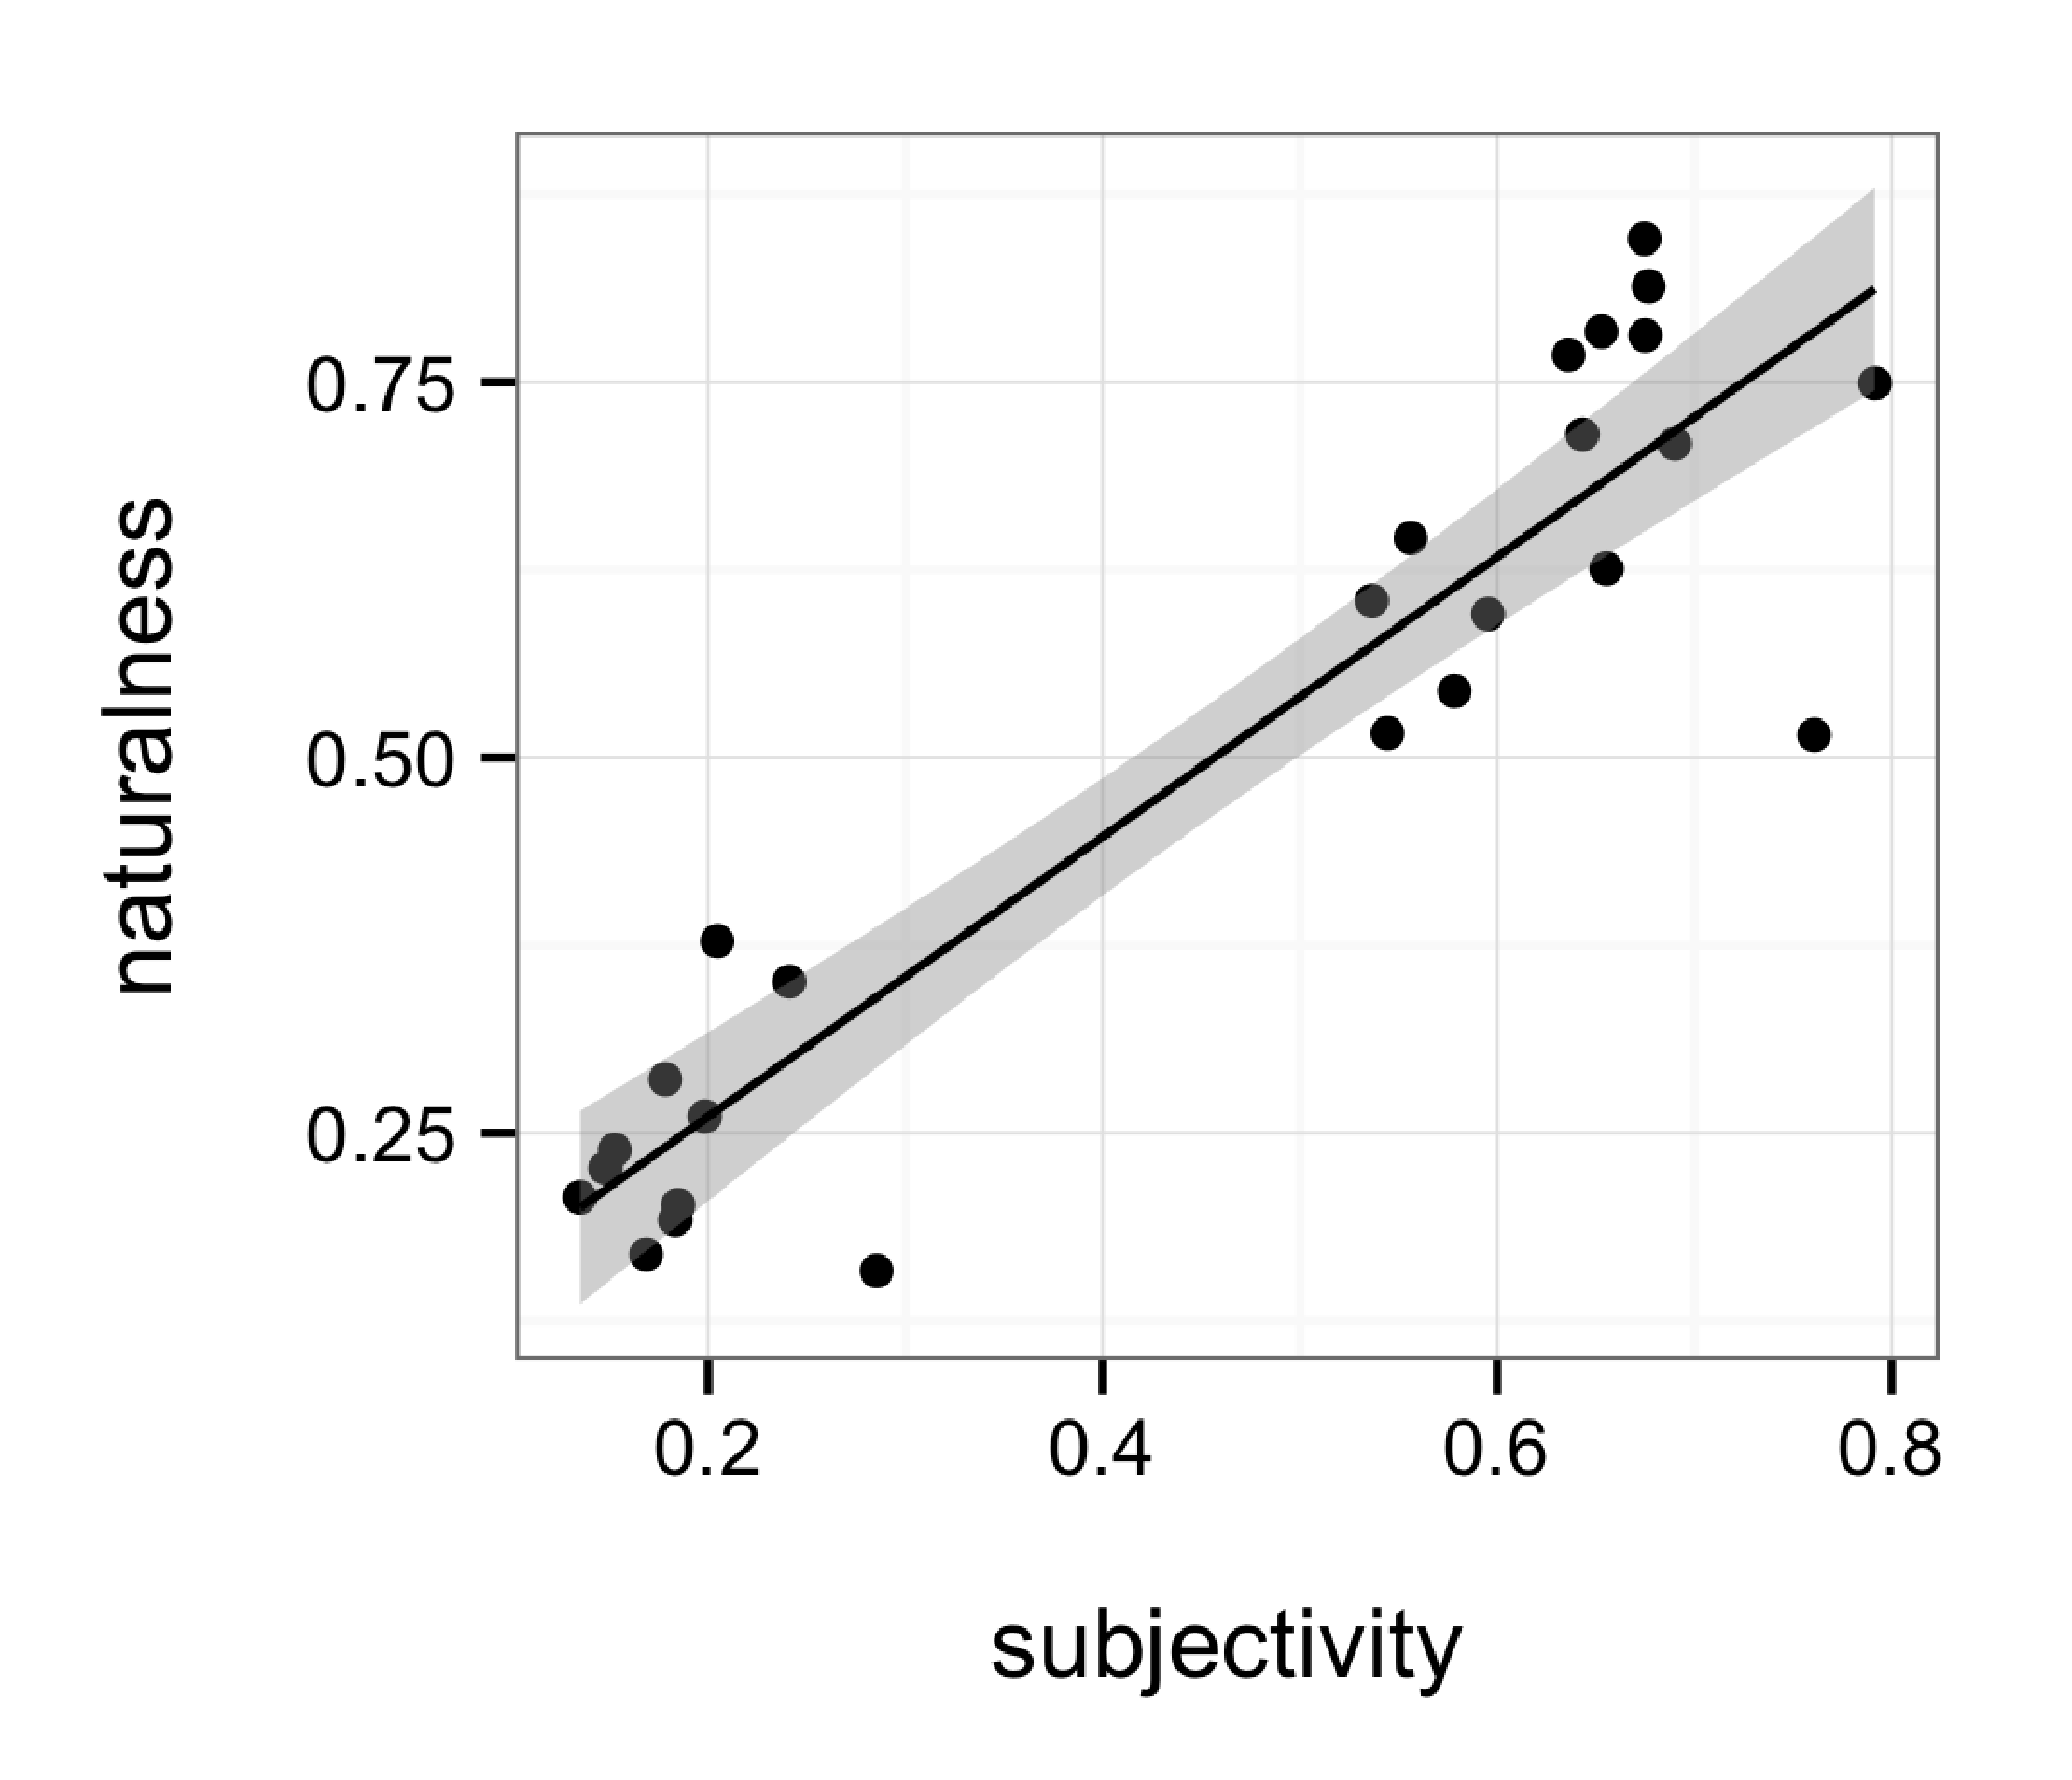
\includegraphics[width=3.5in]{plots/naturalness-subjectivity-new-nouns.eps}
	\caption{Mean naturalness ratings plotted against mean subjectivity scores for each of the 26 adjectives tested in Expt.~2.}\label{fig:subjectivity}
\end{figure}

\subsection{Discussion}

We  failed to find evidence in support of compositional accounts of ordering preferences, which hold that the most important factor in determining order is whether or not an adjective forms a complex concept with the noun it modifies. Using nouns chosen to maximize the probability of complex concepts formed with our 26 adjectives, we failed to find evidence that adjective ordering preferences depend on the modified noun. We do continue to find that subjectivity predicts ordering preferences.
It is quite possible that noun-effects (and hence effects of concept composition) would be found with a different set of adjectives. 
However, this already suggests that the effect of modified nouns explains only a small part of the overall story of adjective order; subjectivity seems to do better.



\section{Operationalizing concept-formability}

Suppose the fundamental factor in predicting adjective ordering is whether an adjective is used to form a complex concept/subkind description or not.

We find this hypothesis intriguing---perhaps concept-formability indeed determines ordering preferences (and therefore correlates with subjectivity)?
We set out to test the hypothesis; as with the studies in our paper, the work lies in operationalizing an abstract notion like whether or not an adjective tends to form a complex concept. The literature on the topic (McNally and Boleda, 2004; Svenonius, 2008) presupposes that intuitions about concept formability are systematic and generalizable; the closest we found in these papers to a proposal for an empirical measure of this factor is the following distinction.

According to McNally and Boleda, the key issue is one of entailment. When an adjective modifies a noun intersectively, the objects described hold both the property named by the noun and the property named by the adjective: a ``male architect'' is both male and an architect (McNally and Boleda, 2004:179, ex.~2). When an adjective and a noun combine to form a complex concept (i.e., a subkind description), the objects described hold the property named by the noun, but not necessarily the property named by the adjective; the modification is (ostensibly) subsective. The authors give the Catalan example \emph{arquitecte t\`{e}cnic} ``technical architect,'' which names architects but not necessarily technical things (McNally and Boleda, 2004:179, ex.~1; cf.~the discussion of \emph{wild rice} in Svenonius 2008). 
Using our original set of materials, we tested whether the objects named by an adjective-noun description hold 1) the property named by the adjective, and 2) the property named by the noun.\footnote{The full experiment is \href{http://web.stanford.edu/~scontras/adjective_ordering/experiments/9-concept-formability/concept-formability.html}{viewable online here}.} We tested 40 participants on Mechanical Turk. 


The semantic analysis given by these authors to adjectives that form complex concepts requires them to compose first with nouns, before run-of-the-mill intersective adjectives; thus, the fundamental factor in predicting adjective ordering ought to be whether an adjective forms a complex concept. Does concept-formability predict ordering preferences?
The adjective concept-formability ratings predict 8\% of the variance in our preference data (r$^{2}=0.08$; 95\% CI [0.00,  0.33]). The noun ratings predict 36\% of the variance (r$^{2}=0.36$; 95\% CI [0.07,  0.62]). Recall that at its worst, subjectivity predicts 70\% of the variance in our preference data.
While it is quite possible that concept-formability plays an important role for some cases (such as \emph{arquitecte t\`{e}cnic}), we did not see evidence that it was critical to ordering preferences in our broad set of items. We chose not to include this null result in our revision, given the brevity of the paper, and the difficulty of validating our measure of concept-formability. 
However, we do include references to and discussion of the relevant literature. 




\bibliographystyle{chicago} 
\bibliography{adjectives}


\end{document}










Compositional (i.e., semantic) accounts of ordering preferences hold that the fundamental factor in predicting adjective ordering is whether or not an adjective is used to form a complex concept/subkind description: first you form the concept, then you modify it with additional adjectives (McNally and Boleda, 2004; Svenonius, 2008).\footnote{Bouchard 2005 makes a similar claim, namely that the formation of complex concepts can override adjective ordering preferences.} 
This would imply that an interaction between the noun and a modifying adjective---whether they combine to form a complex concept---should have a large influence on adjective ordering. 
Indeed, a more general hypothesis is that \emph{some} interaction between a noun and adjective will influence how closely the adjective is placed to that noun. This interaction could be caused by concept-formation, differential subjectivity, or other factors. We tested for such an interaction in our original naturalness ratings and found that noun-specific naturalness did not explain any variance in ordering preference above and beyond adjective-level naturalness. However, there were two adjective-noun pairs in our data with trends in the predicted direction: the naturalness ratings for \emph{hard} and \emph{soft} suggested a preference to occur closer to the noun \emph{cheese}. (Plausibly because hard and soft cheeses are complex concepts.) While these adjective-noun interactions do not survive correction for multiple comparisons in our statistical analysis, they do indicate that a different set of materials might reveal by-noun effects on ordering preference. To follow up on this possibility, we re-ran our order preference and subjectivity experiments with a new set of materials that were chosen to maximize the probability of noun effects.


\section*{Experiment S1: Ordering preferences}

This experiment was a direct replication of our original naturalness ratings experiment (Experiment 1), using a different set of nouns. We chose nouns that we expected to form complex concepts with the given adjectives and therefore yield effects on ordering preferences.

\paragraph{Participants.}

We recruited 50 participants through Amazon.com's Mechanical Turk crowd-sourcing service. Participants were compensated for their participation.

\paragraph{Design and methods.}

The design was identical to our original naturalness ratings experiment: participants were asked to indicate which of two object descriptions sounded more natural, using a sliding scale. Each description featured a noun modified by two adjectives; description pairs contained the same words with the relative adjective order reversed (e.g., ``the big blue thing'' vs.~``the blue big thing''). Adjectives were chosen at random from the original set of 26. The nouns were a smaller set of five (compared to the original ten). Nouns were chosen to maximize the probability of detecting noun-specific effects on adjective ordering preferences. In particular, we expected that nouns that are likely to form complex concepts should be 
highly collocational with that adjective. We thus searched for nouns that occur in particular adjective-noun phrases more frequently than predicted by the individual noun and adjective probabilities; in other words, nouns whose adjective-noun combinations were under-predicted by their individual word probabilities. 

To find these nouns, we estimated the probability $p(A)$ of each adjective from our set of 26 by computing its relative frequency in an adjective-noun sequence in the BNC. We then computed the relative frequency of each noun $p(N)$ occurring in an adjective-noun sequence. Finally, we estimated the predicted joint probability of each adjective-noun combination by taking the product of each individual probability estimate: $\hat{p}(A,N) = p(A)\cdot p(N)$. Comparing  $\hat{p}(A,N)$ to the empirically estimated $p(A,N)$ establishes which adjective-noun combinations are under-predicted---more collocational---and thus likely to name complex concepts. We then restricted nouns to those 50 that maximize the observed range of under-predictedness while simultaneously requiring that each noun be attested to occur with at least 11 of the 26 adjectives; from these 50 nouns, we selected the following four: \emph{apple, cheese, eyes, hair}. (Recall that \emph{cheese} occurred in our original materials, where it suggested possible by-noun effects with the adjectives \emph{hard} and \emph{soft}.) To these four nouns we added a fifth: \emph{thing}.
While \emph{thing} did not occur in the top 50, it did occur naturalistically with the most adjectives (23) out of the set of 26, thus allowing it to serve as a filler for the various object descriptions. The selected nouns, together with the number of adjectives they occur with, their range of ratios of empirical to predicted joint probabilities, and their minimum / maximum ratios, are shown in Table \ref{tab:nouns}.

\renewcommand\thetable{S.\arabic{table}}
\begin{table}
	\centering
	\begin{tabular}{l c c c c}
		\toprule
		Noun & \# of adjectives & range of ratios & minimum ratio & maximum ratio\\
		\midrule
		thing & 23 & 10.4 & 0.1 & 10.5 \\
		eyes & 18 & 120.6 & 0.12 & 120.7 \\
		hair & 15 & 82.9 & 0.03 & 83.0 \\
		cheese & 13 & 114.0 & 0.4 & 114.4 \\
		apple & 11 & 674.0 & 1.1 & 675.1 \\
		\bottomrule
	\end{tabular}
	\caption{For each chosen noun, the number of adjectives (out of 26) that it occurs with; and for each adjective $A$ that the noun occurs with, the range of ratios $p(A,N) / \hat{p}(A,N)$ (empirical to predicted probability of occurrence); the minimum ratio; and the maximum ratio.}
	\label{tab:nouns}
\end{table}




\paragraph{Results.}

To evaluate the role of specific noun information in determining ordering preferences, we performed the same nested linear model comparison from our original naturalness ratings experiment. The models we compared predicted naturalness ratings either by \textsc{adjective} (i.e., the adjective farthest from the noun) only, or by \textsc{adjective} together with its interaction with \textsc{noun} (i.e., the modified noun).
The model comparison revealed that noun-specific ratings did not explain any additional variance in ordering preference beyond adjective-level ratings ($F(1,225) = 0.93, p < 0.75$).  Thus, we again fail to find evidence of noun-specific effects on ordering preferences, this time in our new materials. 

\section*{Experiment S2: Subjectivity}

We next set out to replicate the finding that subjectivity predicts adjective ordering preferences in our new materials.

\paragraph{Participants.}

We recruited 40 participants through Amazon.com's Mechanical Turk crowd-sourcing service. Participants were compensated for their participation.

\paragraph{Design and methods.}

This experiment was a direct replication of our original faultless disagreement subjectivity experiment (Experiment 3), using the new set of nouns from the previous experiment.

\paragraph{Results.}

To evaluate the power of subjectivity in predicting adjective ordering preferences, we compared our new adjective subjectivity scores to the naturalness ratings collected in the previous experiment. 
Faultless disagreement scores account for  84\% of the variance in the new naturalness ratings ($r^2$ 0.84, 95\% CI [0.64,  0.91]; Fig.~\ref{fig:faultless}). 
As with our original materials, more subjective adjectives are preferred farther from the noun; subjectivity again predicts adjective ordering preferences.


\renewcommand\thefigure{S.\arabic{figure}}
\begin{figure}
	\centering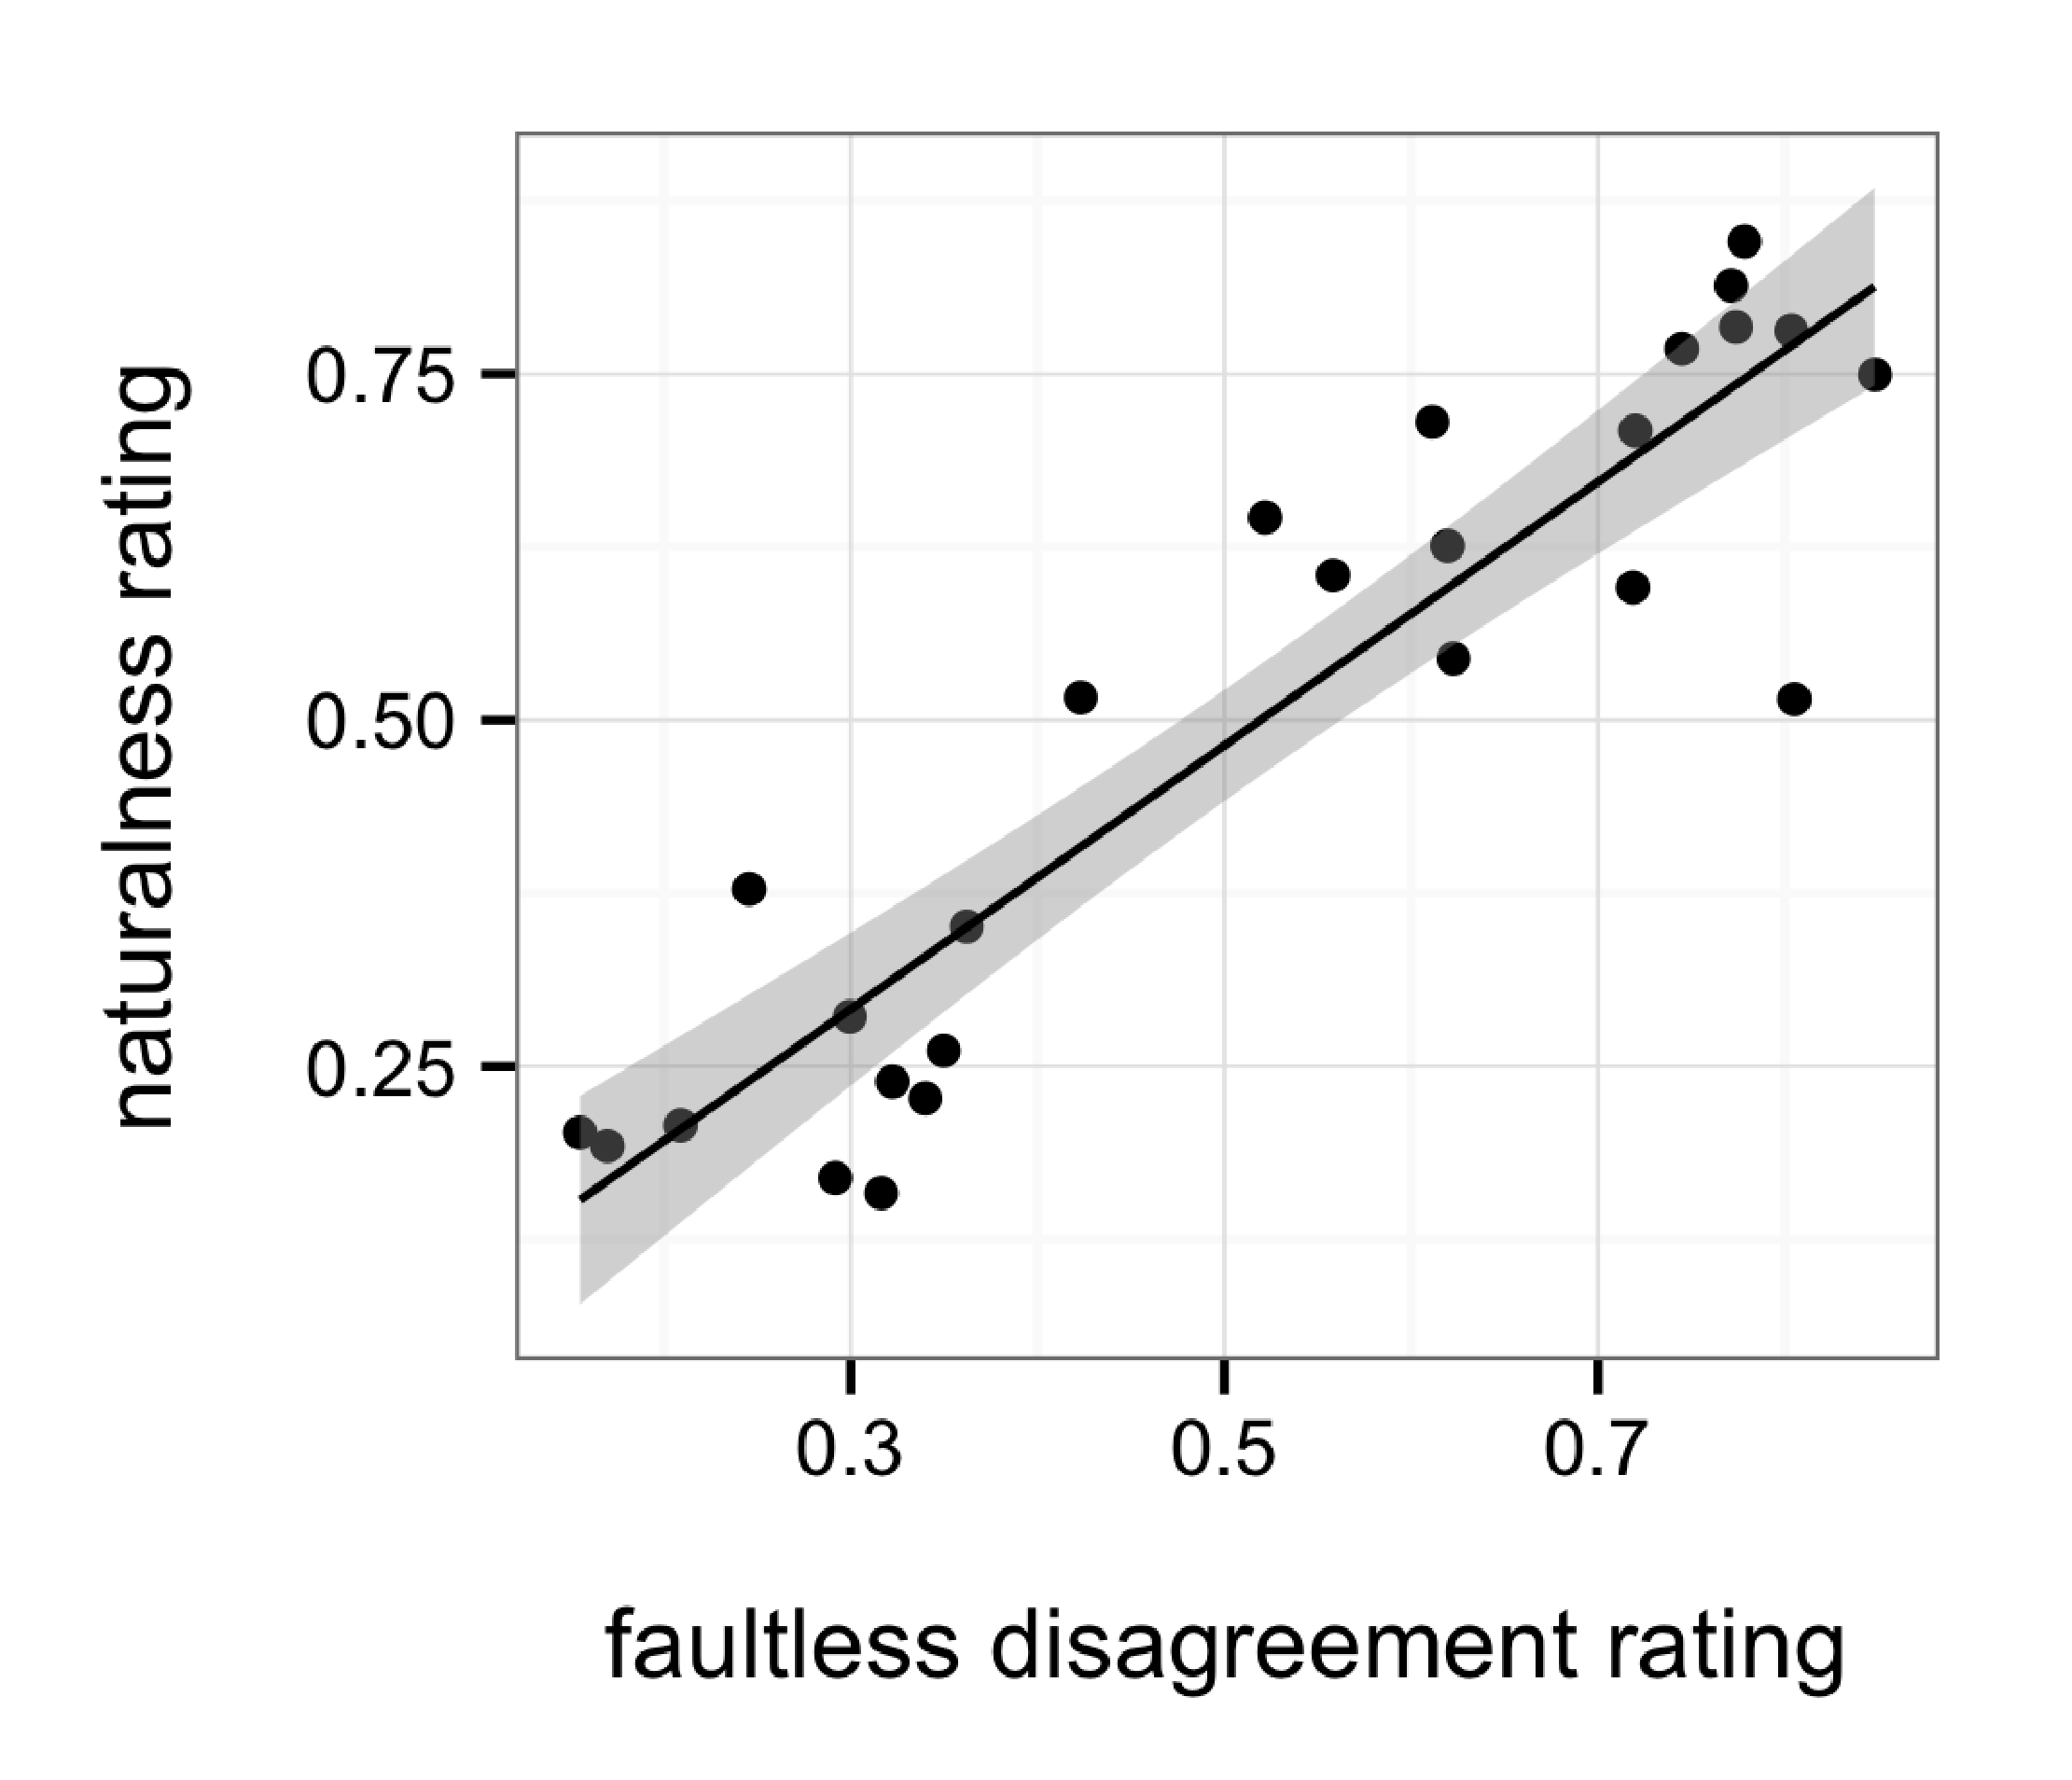
\includegraphics[width=2.8in]{plots/naturalness-faultless-new-nouns.eps}
	\caption{Mean naturalness ratings plotted against mean faultless disagreement scores for each of the 26 adjectives tested.}\label{fig:faultless}
\end{figure}



